\documentclass[12pt]{extreport} % Schriftgröße: 8pt, 9pt, 10pt, 11pt, 12pt, 14pt, 17pt oder 20pt

%% Packages
\usepackage{scrextend}
\usepackage{amssymb}
\usepackage{amsthm}
\usepackage{booktabs}
\usepackage{caption}
\usepackage{subcaption}
\usepackage{chngcntr}
\usepackage{cmap}
\usepackage{color}
\usepackage{csquotes}
\usepackage{enumitem}
\usepackage{float}
\usepackage{graphicx}
\usepackage{hyperref}
\usepackage{ulem}
\usepackage{lmodern}
\usepackage{makeidx}
\usepackage{amsmath}
\usepackage{mathtools}
\usepackage{xpatch}
\usepackage{pgfplots}
\pgfplotsset{compat=1.12}
\usepgfplotslibrary{fillbetween}
\usepackage{amsfonts}
\usetikzlibrary{calc}	
\usetikzlibrary{matrix}	
\usepackage{fancyhdr}
\usepackage{epstopdf}



% Language Setup (English)
\usepackage[utf8]{inputenc} 
\usepackage[T1]{fontenc} 
\usepackage[ngerman]{babel}

% Options
\makeatletter%%  
  % Linkfarbe, {0,0.35,0.35} für Türkis, {0,0,0} für Schwarz, {1,0,0} für Rot, {0,0,0.85} für Blau
  \definecolor{linkcolor}{rgb}{0,0.35,0.35}
  % Zeilenabstand für bessere Leserlichkeit
  \def\mystretch{1.2} 
  % Publisher definieren
  \newcommand\publishers[1]{\newcommand\@publishers{#1}} 
  % Enumerate im 1. Level: \alph für a), b), ...
  \renewcommand{\labelenumi}{\alph{enumi})} 
  % Enumerate im 2. Level: \roman für (i), (ii), ...
  \renewcommand{\labelenumii}{(\roman{enumii})}
  % Zeileneinrückung am Anfang des Absatzes
  \setlength{\parindent}{0pt} 
  % Für das Proof-Environment: 'Beweis:' anstatt 'Beweis.'
  \xpatchcmd{\proof}{\@addpunct{.}}{\@addpunct{:}}{}{} 
  % Nummerierung der Bilder, z.B.: Abbildung 4.1
  \@ifundefined{thechapter}{}{\def\thefigure{\thechapter.\arabic{figure}}} 
  % Chapter-Nummerierung beginnen bei (0):
  \setcounter{chapter}{0}
  % Chapter-Nummerierung
  \renewcommand\thechapter{\Roman{chapter}}
\makeatother%

% Meta Setup 
\title{Globale Optimierung - Sonderübung I}
\author{Kostorz, Belica}
\date{Sommersemester 2017}
\publishers{Karlsruher Institut für Technologie}

%% Math. Definitiones
\newcommand{\C}{\mathbb{C}}
\newcommand{\N}{\mathbb{N}}
\newcommand{\Q}{\mathbb{Q}}
\newcommand{\R}{\mathbb{R}}
\newcommand{\Z}{\mathbb{Z}}
\newcommand{\DO}[1]{\mathcal{D}\left( {#1} \right)}
\newcommand{\RO}[1]{\mathcal{R}\left( {#1} \right)}

\newtheoremstyle{named}{}{}{\normalfont}{}{\bfseries}{:}{0.25em}{#2 \thmnote{#3}}
\newtheoremstyle{nnamed}{}{}{\normalfont}{}{\bfseries}{:}{0.25em}{\thmnote{#3}}
\newtheoremstyle{itshape}{}{}{\itshape}{}{\bfseries}{:}{ }{}
\newtheoremstyle{normal}{}{}{\normalfont}{}{\bfseries}{:}{ }{}
\renewcommand*{\qed}{\hfill\ensuremath{\square}}

\theoremstyle{named}
\newtheorem{unnamedtheorem}{Theorem} \counterwithin{unnamedtheorem}{chapter}
\theoremstyle{nnamed}
\newtheorem*{unnamedtheorem*}{Theorem} 

\theoremstyle{itshape}
\newtheorem{definition}[unnamedtheorem]{Definition}

\theoremstyle{normal}
\newtheorem*{recall}{Recall}
\newtheorem*{example}{Example}
\newtheorem*{theorem}{Theorem}
\newtheorem*{remark}{Remark}
\newtheorem*{satz}{Satz}
\newtheorem*{bemerkung}{Bemerkung}



\fancypagestyle{firststyle}
{
   \fancyhf[C]{\small Globale Optimierung - Sonderübung II - Nadine Kostorz (1972005), Martin Belica (1775706)}
   \fancyfoot[C]{}
}
%% Template
\makeatletter%
\DeclareUnicodeCharacter{00A0}{ } \pgfplotsset{compat=1.7} \hypersetup{colorlinks,breaklinks, urlcolor=linkcolor, linkcolor=linkcolor, pdftitle=\@title, pdfauthor=\@author, pdfsubject=\@title, pdfcreator=\@publishers}\DeclareOption*{\PassOptionsToClass{\CurrentOption}{report}} \ProcessOptions \def\baselinestretch{\mystretch} \setlength{\oddsidemargin}{0.125in} \setlength{\evensidemargin}{0.125in} \setlength{\topmargin}{0.5in} \setlength{\textwidth}{6.25in} \setlength{\textheight}{8in} \addtolength{\topmargin}{-\headheight} \addtolength{\topmargin}{-\headsep} \def\pulldownheader{ \addtolength{\topmargin}{\headheight} \addtolength{\topmargin}{\headsep} \addtolength{\textheight}{-\headheight} \addtolength{\textheight}{-\headsep} } \def\pullupfooter{ \addtolength{\textheight}{-\footskip} } \def\ps@headings{\let\@mkboth\markboth \def\@oddfoot{} \def\@evenfoot{} \def\@oddhead{\hbox {}\sl \rightmark \hfil \rm\thepage} \def\chaptermark##1{\markright {\uppercase{\ifnum \c@secnumdepth >\m@ne \@chapapp\ \thechapter. \ \fi ##1}}} \pulldownheader } \def\ps@myheadings{\let\@mkboth\@gobbletwo \def\@oddfoot{} \def\@evenfoot{} \def\sectionmark##1{} \def\subsectionmark##1{}  \def\@evenhead{\rm \thepage\hfil\sl\leftmark\hbox {}} \def\@oddhead{\hbox{}\sl\rightmark \hfil \rm\thepage} \pulldownheader }	\def\chapter{\cleardoublepage  \thispagestyle{plain} \global\@topnum\z@ \@afterindentfalse \secdef\@chapter\@schapter} \def\@makeschapterhead#1{ {\parindent \z@ \raggedright \normalfont \interlinepenalty\@M \Huge \bfseries  #1\par\nobreak \vskip 40\p@ }} \newcommand{\indexsection}{chapter} \patchcmd{\@makechapterhead}{\vspace*{50\p@}}{}{}{}\def\Xint#1{\mathchoice
    {\XXint\displaystyle\textstyle{#1}} {\XXint\textstyle\scriptstyle{#1}} {\XXint\scriptstyle\scriptscriptstyle{#1}} {\XXint\scriptscriptstyle\scriptscriptstyle{#1}} \!\int} \def\XXint#1#2#3{{\setbox0=\hbox{$#1{#2#3}{\int}$} \vcenter{\hbox{$#2#3$}}\kern-.5\wd0}} \def\dashint{\Xint-} \def\Yint#1{\mathchoice {\YYint\displaystyle\textstyle{#1}} {\YYYint\textstyle\scriptscriptstyle{#1}} {}{} \!\int} \def\YYint#1#2#3{{\setbox0=\hbox{$#1{#2#3}{\int}$} \lower1ex\hbox{$#2#3$}\kern-.46\wd0}} \def\YYYint#1#2#3{{\setbox0=\hbox{$#1{#2#3}{\int}$}  \lower0.35ex\hbox{$#2#3$}\kern-.48\wd0}} \def\lowdashint{\Yint-} \def\Zint#1{\mathchoice {\ZZint\displaystyle\textstyle{#1}}{\ZZZint\textstyle\scriptscriptstyle{#1}} {}{} \!\int} \def\ZZint#1#2#3{{\setbox0=\hbox{$#1{#2#3}{\int}$}\raise1.15ex\hbox{$#2#3$}\kern-.57\wd0}} \def\ZZZint#1#2#3{{\setbox0=\hbox{$#1{#2#3}{\int}$} \raise0.85ex\hbox{$#2#3$}\kern-.53\wd0}} \def\highdashint{\Zint-} \DeclareRobustCommand*{\onlyattoc}[1]{} \newcommand*{\activateonlyattoc}{ \DeclareRobustCommand*{\onlyattoc}[1]{##1} } \AtBeginDocument{\addtocontents{toc} {\protect\activateonlyattoc}} \newcommand{\RightArrow}{\xRightarrow[]{ ~ ~ }} \newcommand{\LeftArrow}{\xLeftarrow[]{ ~ ~ }} \newcommand{\rightArrow}{\xrightarrow[]{ ~ ~ }} \newcommand{\leftArrow}{\xleftarrow[]{ ~ ~ }}
	% Titlepage
	\def\maketitle{ \begin{titlepage} 
			~\vspace{3cm} 
		\begin{center} {\Huge \@title} \end{center} 
	 		\vspace*{1cm} 
	 	\begin{center} {\large \@author} \end{center} 
	 	\vspace*{-0.5cm}
	 	\begin{center} \@date \end{center} 
	 		\vspace*{7cm} 
	 	\begin{center} \@publishers \end{center} 
	 		\vfill 
	\end{titlepage} }
\makeatother%

% Create Index
\makeindex 

\begin{document}

\thispagestyle{empty}

%% Lecture Notes - Start 
\pagenumbering{arabic}\thispagestyle{firststyle}\subsubsection{Aufgabe S.1} \begin{figure}[h!] \centering 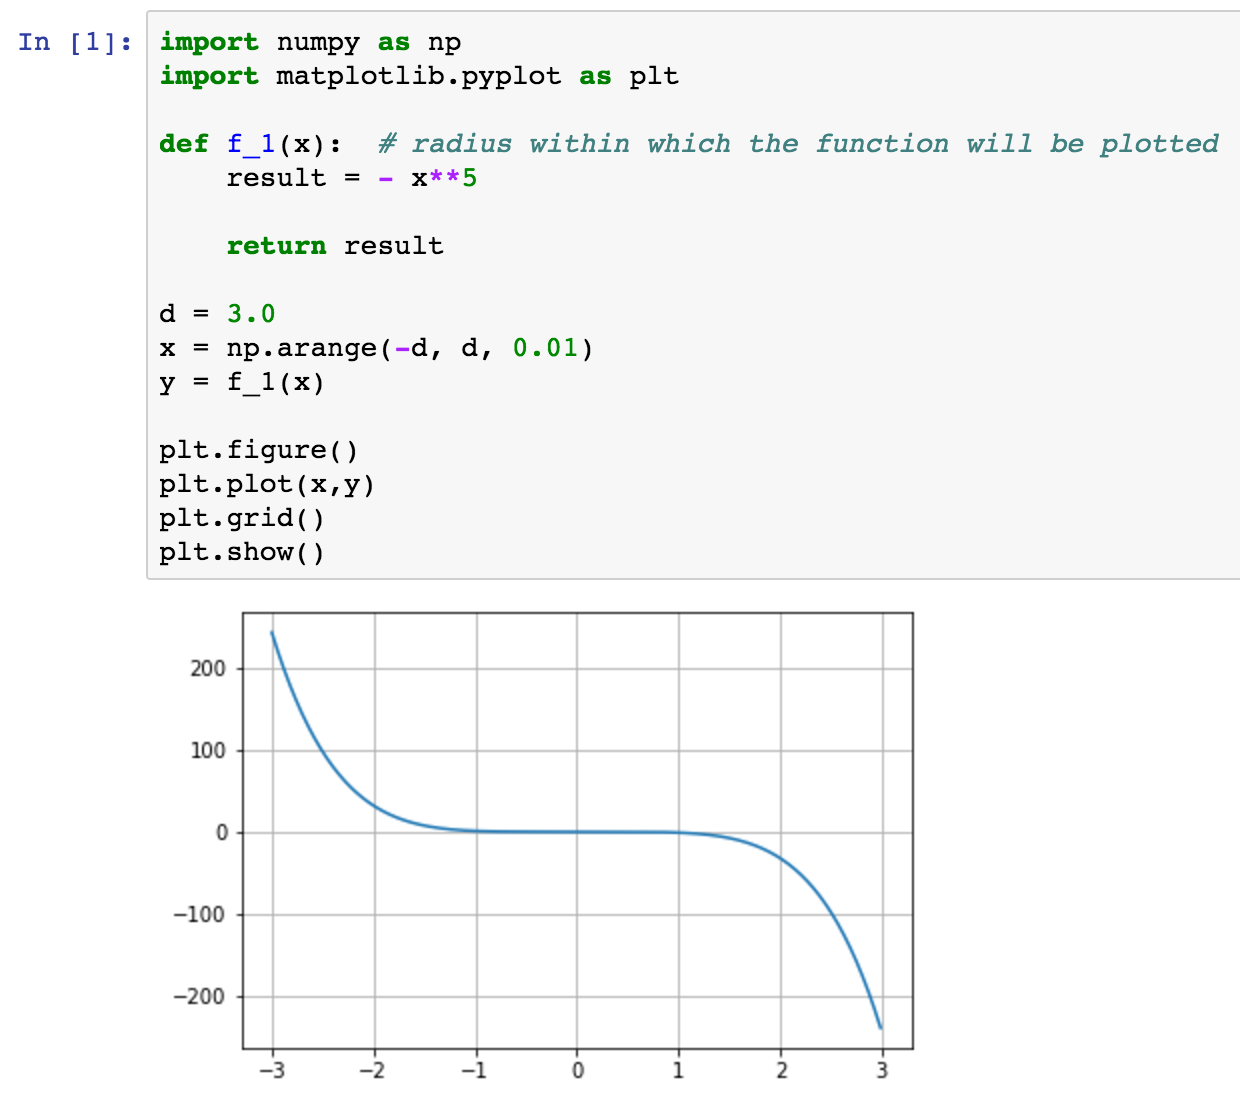
\includegraphics[scale=0.51]{img/sui-i} \label{fig:sub1}\end{figure} \begin{figure}[h!] \centering 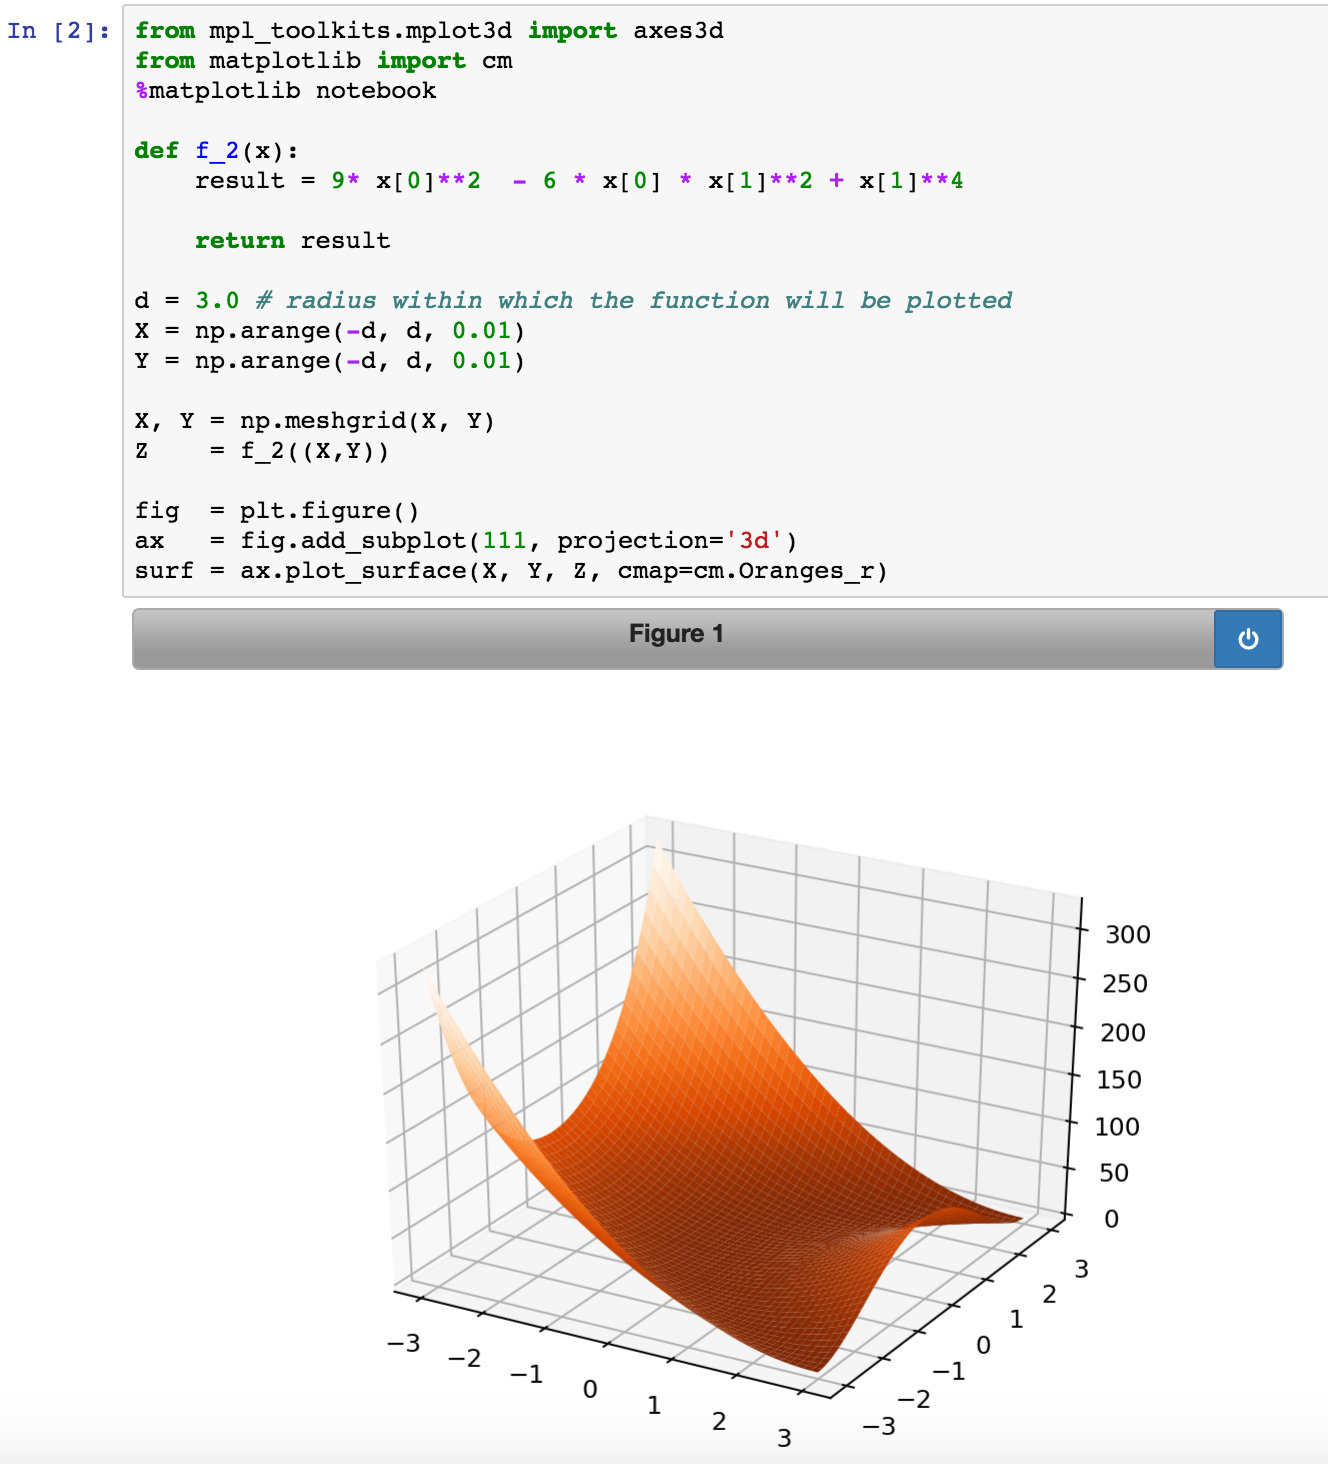
\includegraphics[scale=0.41]{img/sui-ii} \label{fig:sub2}\end{figure}\newpage\subsubsection{Aufgabe S.2} ~\\Gegeben sei das Optimierungsproblem$$ P: \quad \min f(x), \text{ s.t. } x \in M $$mit\begin{enumerate}\item $f(x) = - x^5$, $M =(- \infty, 1)$.\item $f(x) = 9 x_1^2 - 6 x_1 x_2^2 + x_2^4$, $M = \R^2$\item $f(x) = \frac{x^T A x}{\| x - b\|_2 + 1}$, mit $A \in \R^{n \times n}$ positiv definit, $b \in \R^n$ und $M = \R^n$.\end{enumerate}Begründen Sie jeweils: ist $f$ koerziv auf $M$? Ist $P$ lösbar? ~\\\textbf{Hinweis}: Nutzen Sie für Aufgabenteil c) die Äquivalenz der Normen im $\R^n$ ~\bigskip\textit{Nach Vorlesung (Definition 1.2.37) gilt:} ~\\\textit{Gegeben seien eine (nicht notwendigerweise abgeschlossene) Menge $M \subseteq \R^n$ und eine Funktion $f \colon M \rightarrow \R$. Falls für alle Folgen $(x^\nu) \subseteq M$ mit $\lim_{\nu \rightarrow \infty} \| x^\nu \| \rightarrow \infty$ und alle konvergenten Folgen $(x^\nu) \subseteq M$ mit $\lim_{\nu} x^\nu \notin M$ die Bedingung}$$ \lim_{\nu \rightarrow \infty} f(x^\nu) = + \infty $$\textit{gilt, dann heißt $f$ koerziv auf $M$.} ~\\\begin{enumerate}\item $f(x) = - x^5$, $M =(- \infty, 1)$: ~\medskip\begin{proof}Beachte $M \subseteq \R$. Es gilt $\overline{M} = (-\infty, 1]$, d.h. $\partial M = \{ 1 \}$. Für die Koerzivität sind demnach alle Folgen $\left( x^\nu \right) \subseteq M$ zu betrachten für die entweder$$ x^\nu \longrightarrow \infty \quad \text{oder} \quad x^\nu \longrightarrow 1 $$gilt. Sei nun $(x^\nu)$ eine Folge für die gilt $x^\nu \rightarrow 1$. Für alle $\epsilon > 0$ existiert demnach ein $m$, sodass:$$ \| x^{\nu_m} - 1 \| < \epsilon, \quad \forall \nu_m > m. $$Daraus ergibt sich:\begin{align*} \lim_\nu f(x^\nu) = \lim_{\nu \rightarrow \infty} \left( - \left(x^\nu \right)^5 \right) & = - \lim_\nu \left( \left(x^\nu - 1 + 1 \right)^5 \right) \\ & \leq \left| - \lim_{\nu \rightarrow \infty} \left( \left( \| x^\nu -1 \| + 1 \right)^5 \right) \right| \\ & < \lim_{\nu \rightarrow \infty} \left( \epsilon + 1 \right)^5. \end{align*}Da diese Ungleichung im Grenzwert für alle $\epsilon > 0$ gilt, ist $f$ nicht koerziv. ~\\ Die Funktion $f$ ist monoton fallend auf $M$ und streng monoton fallend auf $(0, 1)$, da$$ f'(x) = - 5 x^4 \leq 0 $$mit strikter Ungleichung für $x \neq 0$. Damit ist $$ \inf_{x \in M} f(x) = \lim_{x \rightarrow 1} f(x) = -1. $$Da das Infimum aber nicht in der Menge angenommen wird ($M$ offen, damit ist aufgrund strenger Monotonie $f(x) > -1$ für alle $x \in M$), ist das Problem nach Definition 1.2.3 nicht lösbar. \end{proof}\item $f(x) = 9 x_1^2 - 6 x_1 x_2^2 + x_2^4$, $M = \R^2$:\begin{proof}Es gilt$$ f(x) = 9 x_1^2 - 6 x_1 x_2^2 + x_2^4 = (3 x_1 - x_2^2)^2. $$Für jede Folge für die für alle $\nu \in \N$ gilt dass $\sqrt{3 x^\nu_1} = x^\nu_2$ folgt:$$ f(x^\nu) = 0 \quad \forall \nu \in \N, $$z.B. $x^\nu = (\nu, \sqrt{3\nu}) ~\forall \nu \in \N \Rightarrow \lim_{\nu \rightarrow \infty} f(x^\nu) = 0$. Da wir eine Folge gefunden haben für die $\| x^\nu \| \rightarrow \infty$ aber $\lim_{\nu \rightarrow \infty} f(x^\nu) = 0$ gilt, ist $f$ nicht koerziv. ~\\ Es gilt $f(x) = (3 x_1 - x_2^2)^2 \geq 0 = \inf_{x \in M} f(x)$, wobei $$ f(x) = 0 \iff (3 x_1 - x_2^2)^2 = 0 \iff x_1 = \frac{x_2^2}{3} $$Da es $(x_1, x_2) \in M$ gibt, die die obige Bedingung erfüllen (z.B. $x = \left(\frac{1}{3}, 1\right)$), nimmt $f$ auf $M$ sein Infimum an, und das Problem ist nach Definition 1.2.3. lösbar.\end{proof}\item $f(x) = \frac{x^T A x}{\| x - b\|_2 + 1}$, mit $A \in \R^{n \times n}$ positiv definit, $b \in \R^n$ und $M = \R^n$:\begin{proof}Da $M = \R^{n \times n}$ sei $(x^\nu)$ eine beliebige divergente Folge. Aufgrund der positiven Definitheit von $A$ ist $ x^T A x > 0$ und damit ist\begin{align}f(x) = \frac{x^T A x}{\| x - b\|_2 + 1} > 0. \tag*{$(*)$}\end{align}In der Übung wurde die Norm$$ \| x \|_{\tilde{A}} = \sqrt{\langle x, x \rangle_{\tilde{A}}} = \sqrt{x^T \tilde{A} x} $$eingeführte, mit einer positiv definite, symmetrische Matrix $\tilde{A}$. Sei$$B \coloneqq \frac{A^T + A}{2},$$dann ist $B$ eine positiv definite, symmetrische Matrix und es gilt nach Übung$$ x^T A x = x^T B x. $$Damit folgt:$$ \left| f(x^\nu) \right| = \left| \frac{\left(x^\nu \right)^T A x^\nu }{\| x^\nu - b\|_2 + 1} \right| = \frac{\left\| x^\nu \right\|_{B}^2}{\| x^\nu - b\|_2 + 1}. $$Aufgrund der Divergenz der Folge $(x^\nu)$ gilt für $\nu$ groß genug unter Verwendung der Dreiecksungleichung die Abschätzung\begin{align*} \left| f(x^\nu) \right| = \frac{\left\| x^\nu \right\|_{B}^2}{\| x^\nu - b\|_2 + 1} & \geq \frac{\left\| x^\nu \right\|_{B}^2}{2 \| x^\nu - b\|_2 } \\ & \geq \frac{\left\| x^\nu \right\|_{B}^2}{2 \left( \| x^\nu \|_2 + \| b\|_2 \right)} \\ & \geq \frac{\left\| x^\nu \right\|_{B}^2}{2 \left( \| x^\nu \|_2 + \| x^\nu \|_2 \right)} \end{align*}Durch die Äquivalenz der Normen im $\R^n$ existiert nun eine Konstante $c$ so, dass\begin{align}\left| f(x^\nu) \right| \geq \frac{c}{2} \cdot \frac{\left\| x^\nu \right\|_{B}^2}{2 \left( \| x^\nu \|_B + \| x^\nu \|_B \right)} = \frac{c}{4} \cdot \frac{\left\| x^\nu \right\|_{B}^2}{ \| x^\nu \|_B} = \frac{c}{4} \cdot \| x^\nu \|_B \longrightarrow \infty, \tag*{$(**)$}\end{align}wobei wir im letzten Schritt wieder die Äquivalenz der Normen verwendet haben, da somit $x^\nu$ in allen Normen divergiert. $(*)$ zusammen mit $(**)$ liefert für alle divergenten Folgen $(x^\nu)$, dass $$ f(x^\nu) \longrightarrow \infty, $$d.h. $f$ ist koerziv. ~\\Da $M$ nicht-leer und abgeschlossen, und $f$ stetig und koerziv ist, ist das Problem nach Korollar 1.2.30 lösbar.\end{proof}\end{enumerate}\newpage\subsubsection{Aufgabe S.3} ~\\Gegeben sei das unrestringierte Optimierungsproblem$$ P : \quad \min_{x \in \R^2} \exp \left(- \min \big\{- x_1 - 3, -\left|x_2 - 4\right|, x_1 + x_2 - 20 \big\} \right).$$\begin{enumerate}\item Geben Sie die verallgemeinerte Epigraph-Umformulierung $P_{epi}$ von $P$ an (siehe Übung 1.3.9. im Skript). Begründen Sie, welche Funktionen $f$, $g$, $F$ und $G$ Sie für die Umformulierung verwenden.\begin{proof}Da es sich um ein unrestringiertes Problem handelt, ist $X = \R^2$, $G \equiv 0, g \equiv 0$. Definiere\begin{align*}& F: \R \rightarrow \R, x \mapsto e^{x}, \\& f: \R^2 \rightarrow \R, x \mapsto -\min\big\{- x_1 - 3, -\left|x_2 - 4\right|, x_1 + x_2 - 20\big\}. \\\end{align*}Damit ist das unrestringierte Optimierungsproblem äquivalent zu$$ P : \quad \min_{x \in \R^2} F(f(x)) \text{ s.t. } G(g(x)) \leq 0, x \in X $$Nach Übung 1.3.9 (Verallgemeinerte Epigraph-Umformulierung) ist somit folgende Epigraph-Umformulierung äquivalent zu $P$:$$ P_{epi}: \min_{(x, \alpha, \beta) \in \R^2 \times \R \times \R} F(\alpha) \text{ s.t. } G(\beta) \leq 0, f(x) \leq \alpha, g(x) \leq \beta, x \in X $$$$ \iff \min_{(x, \alpha) \in \R^2 \times \R} e^{\alpha} \text{ s.t. } -\min\big\{- x_1 - 3, -\left|x_2 - 4\right|, x_1 + x_2 - 20\big\} \leq \alpha, ~ x \in X $$Wobei wir im letzten Schritt $\beta$ aufgrund der trivialen Bedingung $G(\beta) \equiv 0 \overset{!}{=} 0$ zur Vereinfachung fallen gelassen haben.\end{proof}\item Formulieren Sie, aufbauend auf Aufgabenteil a), ein lineares Optimierungsproblem $P_{lin}$, welches die selben Optimalpunkte wie $P_{epi}$ besitzt.\begin{proof}Es gilt\begin{align*}f(x) & = -\min\big\{- x_1 - 3, -\left|x_2 - 4\right|, x_1 + x_2 - 20\big\} \\& = ~~ \max\big\{ x_1 + 3, \left|x_2 - 4\right|, -(x_1 + x_2) + 20\big\}. \end{align*} Die Bedingung $f(x) \leq \alpha$ aus der Epigraph-Formulierung bedeutet, dass jede Komponente des Maximums kleiner gleich $\alpha$ sein muss, d.h. das folgende Problem ist äquivalent zu $P_{epi}$:$$ \tilde{P}_{epi}: \min_{(x, \alpha) \in \R^2 \times \R} e^{\alpha} \text{ s.t. } x \in X, \begin{cases} x_1 + 3 \leq \alpha \\ x_2 - 4 \leq \alpha, ~ x_2 - 4 \geq - \alpha \\ -(x_1 + x_2) + 20 \leq \alpha \end{cases} $$ Da die Exponentialfunktion streng monoton ist, ist jedes Minimum der Identität auf dieser Menge gleich dem Minimum der Exponentialfunktion. Ein lineares Optimierungsproblem $P_{lin}$, welches die selben Optimalpunkte wie $P_{epi}$ besitzt, lautet somit$$ {P}_{lin}: \min_{(x, \alpha) \in \R^2 \times \R} \alpha \text{ s.t. } x \in X, \begin{cases} x_1 + 3 \leq \alpha \\ x_2 - 4 \leq \alpha, ~ x_2 - 4 \geq - \alpha \\ -(x_1 + x_2) + 20 \leq \alpha \end{cases} $$ \end{proof}\item Zeigen Sie, mit Hilfe des verschärften Satz von Weierstraß, dass das Problem $P_{lin}$ lösbar ist.\begin{proof}Das Problem $P_{lin}$ ist auf der Menge $$M \subseteq \big\{ (\alpha, x) = (\alpha, (x_1, x_2)) : \alpha \in \R, x \in \R^2 \big\}$$ definiert, die die folgenden Nebenbedingungen hält:$$\begin{cases} x_1 + 3 \leq \alpha \\ x_2 - 4 \leq \alpha, ~ x_2 - 4 \geq - \alpha \\ -(x_1 + x_2) + 20 \leq \alpha \end{cases} $$ Die Funktion $f(\alpha) = \alpha$ ist als Identität stetig. Für den verschärften Satz von Weierstraß bleibt zu zeigen, dass für ein $\beta \in \R$ die Menge $$ \operatorname{lev}_{\leq}^{\beta}(f, M)= \big\{ (\alpha, x) \in M | f(\alpha) = \alpha \leq \beta \big\} $$ nicht-leer und kompakt ist. Für $\alpha < 0$ existiert kein $x_2$, sodass $x_2 - 4 \leq \alpha \text{ und } x_2 -4 \geq - \alpha$. Für $\alpha = 0$, ist $x_2 = 4$ und damit $\not\exists x_1$: $x_1 + 3 \leq 0 \text{ und } - (x_1 + 4) + 20 \leq 0$ Für $\alpha > 0$ ist \begin{align} x_2 \in [4 - \alpha, 4 + \alpha], ~ \tag*{$(*)$}\end{align}d.h. $x_2$ liegt in einer nicht-leeren, abgeschlossenen Menge. Aus den Restriktionen erhalten wir außerdem\begin{align} x_1 \in [20 - x_2 - \alpha, \alpha - 3], ~ \tag*{$(**)$}\end{align}Diese Menge ist für $\alpha > \frac{19}{3}$ nicht leer und abgeschlossen, da für $x_2 = 4 + \alpha$: $$ 20 - x_2 - \alpha < \alpha - 3 \iff 23 - ( 4 + \alpha ) < 2 \alpha \iff \alpha > \frac{19}{3}. $$Somit liefert ein $\beta > \frac{19}{3}$, dass $f(\alpha) = \alpha \in \left[\frac{19}{3}, \beta \right]$ beschränkt ist. Das in Kombination mit $(*)$ bzw. $(**)$ liefert die Beschränktheit von $x_1, x_2$. Zusammengefasst ist für ein $\beta > \frac{19}{3}$ die Menge$$ \big\{ (\alpha, x) \in M | f(\alpha) = \alpha \leq \beta \big\} $$nicht-leer und kompakt und der verschärfte Satz von Weierstraß garantiert die Lösbarkeit des Problems.\end{proof} ~\newpage\item Modellieren Sie das Problem in Matlab/ Jupyter Notebook und geben Sie den globalen Minimalpunkt von $P_{lin}$ aus.\begin{figure}[h!] \centering 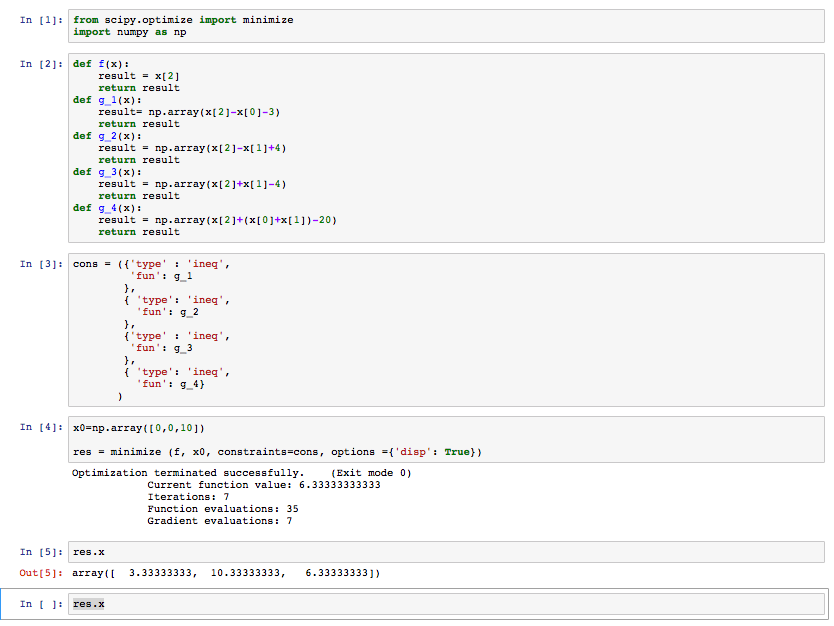
\includegraphics[scale=0.55]{img/suiii-vi} \label{fig:fig3}\end{figure}\item Bestimmen Sie einen globalen Optimalpunkt und den Optimalwert von P.\begin{proof}Die Minimalpunkte von $P$ und $P_{lin}$ stimmen nach Konstruktion überein (siehe 3b), also folgt aus d) für die Optimalpunkte $x^*=(\frac{10}{3}, \frac{31}{3})$.\\Einsetzten in das Ursprungsproblem ergibt: $$f(x^*)= \exp (-\min\left\{ -x_1-3, -|x_2-4|, x_1+x_2-20\right\}) $$$\iff \exp\left(-\min\left\{ \frac{1}{3}, -\frac{19}{3}, -\frac{19}{3} \right\}\right) = \exp( \frac{19}{3}) = 563.0302$\end{proof}\end{enumerate}\newpage\subsubsection{Aufgabe S.4} ~\\Gegeben seien eine $(p, n)$-Matrix $A$, sowie Vektoren $b \in \R^p$ und $a \in \R^n$. In dieser Aufgabe geht es um die Projektion von $a$ auf die Menge$$ \hat{M} \coloneqq \big\{ x \in \R^n \colon A x \leq b \big\}. $$Dieses Problem tritt in ähnlicher Form in der Gemischt-Ganzzahligen Optimierung im Rahmeneines Ansatzes zur heuristischen Bestimmung von Punkten in$$ M = \big\{ x \in \Z^m \colon Ax \leq b \big\} $$auf (Feasibility Pump, [1]). Wählt man für die Projektion die $\ell_1$-Norm, so lässt sich dasOptimierungsproblem formulieren als$$ FP \colon \quad \min_{x \in \R^n} \sum_{j=1}^{n} \left| x_j - a_j \right| \text{ s.t. } Ax \leq b. $$Bestimmen Sie ein äquivalentes lineares Optimierungsproblem $FP_{lin}$, indem Sie die verallgemeinerte Epigraph Umformulierung (vgl. Übung 1.3.9 im Skript) anwenden. Begründen Sie, welche Funktionen $f$, $g$, $F$ und $G$ Sie für die Umformulierung verwenden.\begin{proof}Wir definieren\begin{align*}& f \colon \R^n \rightarrow \R^n, x \mapsto x - a \\& F \colon \R^n \rightarrow \R, x \mapsto \| x \|_1 \\& g \colon \R^n \rightarrow \R^n, x \mapsto Ax - b \\& G \colon \R^n \rightarrow \R, x \mapsto \max \{ x_1, \dotsc, x_n \}\end{align*}Damit gilt für $X = \R^n$, dass das obiges Optimierungsproblem äquivalent dargestellt werden kann durch$$ P: \quad \min_{x \in \R^n} F(f(x)) \text{ s.t. } G(g(x)) \leq 0, x \in X $$$$ \iff \min_{x \in \R^n} \| x - a \|_1 \text{ s.t. } \max_i \{ (Ax - b)_i \} \leq 0, x \in \R^n, $$wobei wir ausnutzen, dass $Ax \leq b \iff Ax -b \leq 0 \iff \max_i \{ (Ax - b)_i \} \leq 0$. Damit sind die Voraussetzungen der verallgemeinerten Epigraph-Formulierung gegeben und diese lautet:$$ P_{epi}: \min_{(x, \alpha, \beta) \in \R^n \times \R^n \times \R^l} F(\alpha) ~ \text{ s.t. } ~ G(\beta) \leq 0, ~ f(x) \leq \alpha, ~ g(x) \leq \beta, ~ x \in X $$ $$ \iff \min_{(x, \alpha, \beta) \in \R^n \times \R^n \times \R^l} \sum_{i=1}^n |\alpha_i| ~ \text{ s.t. } ~ x \in X,~ \begin{cases} \beta_i \leq 0, \\ (x - a)_i \leq \alpha_i, \\ (Ax - b)_i \leq \beta_i, \end{cases} \forall i \in \{1, \dotsc, n \} $$was ein lineares Problem darstellt.\end{proof}\newpage\subsubsection{Aufgabe S.5} ~\\Skizzieren Sie folgende Mengen $M \subseteq \R^2$und zeigen oder widerlegen Sie jeweils die Konvexität von $M$. ~\\ ~\\\textit{Definition 2.1.1.: Eine Menge $M \subseteq \R$ heißt konvex, falls folgendes gilt}$$ \forall x, y \in M, \lambda \in (0, 1): (1-\lambda)x + \lambda y \in M $$\textit{(d.h. die Verbindungsstrecke von je zwei beliebigen Punkten in $M$ gehört komplett zu $M$).}\begin{enumerate}\item $M \colon \big\{ x \in \R^2 \colon \left( x_1 - 1 \right)^2 + \left( x_2 - 1 \right)^2 \leq 4 \big\}$\begin{proof}Sei $f(x) \coloneqq \left( x_1 - 1 \right)^2 + \left( x_2 - 1 \right)^2 - 4$, dann ist $$ M = f_{\leq}^{0}. $$Da $f$ als Polynom zweimal stetig differenzierbar ist, ist die Hesse-Matrix wohldefiniert:$$ \nabla f(x) = \left(\begin{array}{c} 2x_1 - 2 \\ 2 x_2 -2 \end{array}\right) \Rightarrow D^2 f(x) =\left(\begin{array}{rr} 2 & 0 \\ 0 & 2 \end{array}\right) . $$ Die charakteristische Gleichung für $D^2 f(x)$ lautet somit: $$\det (D^2 f(x) - \lambda I) = (2-\lambda)^2 \overset{!}{=} 0.$$ Damit ist $\lambda = 2$ zweifacher Eigenwert, womit $f$ konvex ist. Nach Übung 4.4 ist damit $M$ eine konvexe Menge.\begin{figure}[h!] \centering 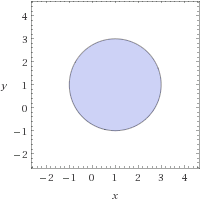
\includegraphics[scale=0.55]{img/suv-i} \label{fig:fig1}\end{figure}\end{proof} \item $M \colon \big\{ x \in \R^2 \colon \left( x_1 - 1 \right)^2 + \left( x_2 - 1 \right)^2 \leq 4, \left( x_1 - 3 \right)^2 + \left( x_2 - 1 \right)^2 \geq 1 \big\}$\begin{proof}Behauptung: $M$ ist nicht konvex, da $x,y \in M$ existieren, deren konvexe Verbindungsstrecke nicht komplett in der Menge liegt. ~\\Sei hierfür $x=(\frac{11}{4}, 1-\frac{\sqrt{15}}{4})$ und $y=(\frac{11}{4}, 1+\frac{\sqrt{15}}{4})$, dann gilt $x,y\in M$. Wähle konkret $\lambda=0,5$ und definiere $z \coloneqq (1-\lambda)x+\lambda y$. Wäre $M$ konvex, so müsste folgen $z \in M$. Einsetzen der obigen Werte ergibt:\begin{align*}z_1 & = 0,5*\frac{11}{4}+(1-0.5)\frac{11}{4}= \frac{11}{4} \\z_2 & = (0,5*(1-\frac{\sqrt{15}}{4})+(1-0.5)(1+\frac{\sqrt{15}}{4})= 1\end{align*}Einsetzen der Werte in die Ungleichungen ergibt: \\\begin{align*}(z_1-1)^2+(z_2-1)^2 & = \frac{49}{16} \leq 4 \\(z_1-3)^2+(z_2-1)^2 & = \frac{1}{16} \leq 1 \end{align*}Aufgrund der 2. Ungleichung gilt $z \notin M $ und damit ist $M$ nicht konvex. ~\\\begin{figure}[h!] \centering 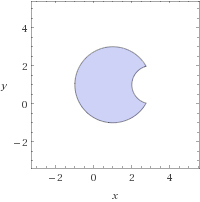
\includegraphics[scale=0.55]{img/suv-ii} \label{fig:fig2}\end{figure}\end{proof} ~\newpage\item $M \colon \big\{ x \in \R^2 \colon \left( x_1 - 1 \right)^2 + \left( x_2 - 1 \right)^2 \leq 4, \left( x_1 - 3 \right)^2 + \left( x_2 - 1 \right)^2 \geq 16 \big\}$\begin{proof}Behauptung: Die Menge $M$ enthält nur den Punkt $(-1, 1)$ und ist damit trivialerweise konvex. Betrachte hierfür die Randbedingungen\begin{align}\left( x_2 - 1 \right)^2 \leq 4 - \left( x_1 - 1 \right)^2 \text{ und } \left( x_2 - 1 \right)^2 \geq 16 - \left( x_1 - 3 \right)^2. \tag*{$(*)$}\end{align} Einsetzen ineinander liefert$$ 4 - \left( x_1 - 1 \right)^2 \geq 16 - \left( x_1 - 3 \right)^2 \iff 8 - 4x_1 \geq 12 \iff x_1 \leq -1 $$Da allerdings $$ 4 \geq \left( x_1 - 1 \right)^2 + \left( x_2 - 1 \right)^2 \geq (x_1 - 1)^2, $$ die zwei Möglichkeiten $x_1 \leq 3$ und $-1 \geq x_1$ liefert, erfüllt nur $x_1 = -1$ die Bedingung. Aus $(*)$ folgt damit direkt $$ 4 - (x_1 - 1)^2 = 0 \geq \left( x_2 - 1 \right)^2 \geq 0 \iff x_2 = 1 $$und somit die Behauptung. ~\\\begin{figure}[h!] \centering 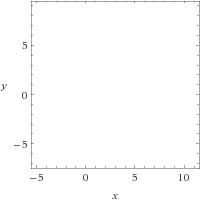
\includegraphics[scale=0.45]{img/suv-iii} \label{fig:fig3}\end{figure}\end{proof}\end{enumerate} 
\end{document} 